\documentclass[../pflichtenheft.tex]{subfiles}

\begin{document}

\clearpage

\section{Zielbestimmung}
	Das Ziel des Projektes ist es, zwei \Gls{library}en und eine \Gls{app} zu entwickeln. Jede davon stellt eine eigene Komponente dar.
	\begin{itemize}
		\item Mit \Gls{komp1} (Sensor Bibliothek) sollen \Gls{developer} \Gls{sensordata} der \Gls{earable}s auslesen können.
		\item Weiterhin soll \Gls{komp2} (Schritterkennungs Bibliothek) \Gls{stepdata} aus den \Gls{sensordata} extrahieren.
		\item \Gls{komp3} (\Gls{app}) soll dann einige Funktionen der ersten beiden Komponenten auch für \gls{user} verfügbar machen.
	\end{itemize}
	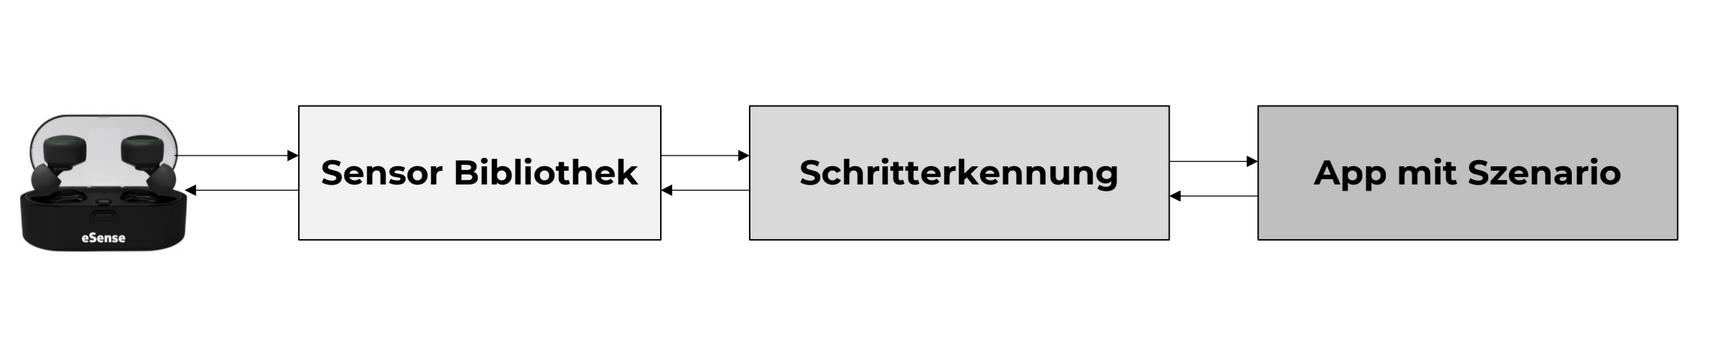
\includegraphics[page=1,width=400pt,keepaspectratio]{../graphics/Praeambel/YHB_Project_Pic.png}
	\subsection{Musskriterien}
		\begin{itemize}
			\item \Gls{komp1} muss \Gls{sensordata} der \Gls{earable}s auslesen können
			\item \Gls{komp1} muss \Gls{audiodata} an die \Gls{earable}s senden können
			\item \Gls{komp2} muss - mithilfe der von \Gls{komp1} erlangten \Gls{sensordata} - Schritte erkennen, während der \Gls{user} geht oder läuft
			\item \Gls{komp3} muss eine \Gls{bc}- sowie eine \Gls{ble}-Verbindung zu ausgewählten \Gls{earable}s aufbauen können
			\item \Gls{komp3} muss Verknüpfungen zu verschiedenen \gls{audiofile}en in einer lokalen, vom \Gls{user} bearbeitbaren \Gls{audiolib} speichern können
			\item \Gls{komp3} muss aus der \Gls{audiolib} ein zur Schrittfrequenz passendes Lied aussuchen können (Motivationsmusik-Modus)
			\item \Gls{komp3} muss \gls{audiofile}en der \Gls{audiolib} über die \Gls{earable}s wiedergeben können
			\item \Gls{komp3} muss ausgewählte, von \Gls{komp1} und \Gls{komp2} gewonnene Daten, anzeigen können: Gerätename und Akkuzustand der \Gls{earable}s
			\item Alle Komponenten müssen auf \Gls{device}en mit \gls{ios} oder \Gls{android} nutzbar sein
			\item \Gls{i18n} (Deutsch und Englisch) soll unterstützt werden
		\end{itemize} 
	\subsection{Wunschkriterien}
		\begin{itemize}
			\item \Gls{komp1} soll die Konfiguration der \Gls{earable}s verwalten können
			\item \Gls{komp2} soll Schritte protokollieren, um eine nachträgliche Auswertungen anzubieten (Zum Beispiel in Form von Diagrammen)	
			\item \Gls{komp3} soll die Schrittanzahl anzeigen und der \Gls{user} diese zurücksetzen, als auch den Gerätenamen ändern können
			\item \Gls{komp3} soll einen weiteren Modus erhalten, welcher die Musik beim Stehenbleiben stoppt (AutoStop-Modus)
			\item \Gls{komp3} soll es möglich sein, den \Gls{bpm}-Wert einer \gls{audiofile} automatisch (unter Zuhilfename einer externen \Gls{library}) zu ermitteln
			\item Es soll die \Gls{spotify} \Gls{api} verwendet werden, um ein Lied mit passendem \Gls{bpm}-Wert in einer \Gls{spotify} \Gls{playlist} des \Gls{user}s zu finden und dieses wiederzugeben
			\item Der \Gls{user} soll \Gls{komp3} weitere Sprachen in Form von Sprachdateien (.lang) hinzufügen können
		\end{itemize}
	\subsection{Abgrenzungskriterien}
		\begin{itemize}
			\item Keine der Komponenten muss auf anderen Betriebssystemen als den explizit geforderten lauffähig sein (Zum Beispiel Windows Phone)
			\item Außer \quote{\gls{esense}} werden keine weiteren \Gls{earable}-Plattformen unterstützt
			\item \Gls{komp3} muss von sich aus keine Musik anbieten
			\item \Gls{komp1} kann nicht das Mikrophon der Kopfhörer ansteuern
			\item Es kann sich nicht mit mehreren \Gls{earable}s auf einmal verbunden werden
		\end{itemize}

\end{document}
